\documentclass[11pt, letterpaper]{article}
\usepackage[utf8]{inputenc}
\usepackage[letterpaper, margin=1in]{geometry}
\usepackage{amsmath}
\usepackage{amssymb}
\usepackage{amsthm}
\usepackage{graphicx}
\usepackage[font=scriptsize]{caption}
\usepackage{subcaption}
\graphicspath{ {.} }
\captionsetup{justification=raggedright, singlelinecheck=false}


\title{Homework 4}
\author{Ryan Tang}
\date{November 3rd 2022}

\begin{document}
\maketitle

\section{Exercise 17.3}
Here we have a Hidden Markov Model (HMM) with a Gaussian Mixture observation model. Assuming we have a discrete $Z \in \{1 \dots K\}$ latent states in the HMM model and an observation model comprised of $M = 1,2... $ mixture of Gaussians. Let $i, k$ be the indexers for $Z$, and $m$ be the indexer for $M$, and we define the transition matrix $A = [A_{jk}]$ be a square matrix that is in $R^{K \times K}$ with each row $A_j = \sum_k A_{jk} = 1$. $A$ is time-invariant because of a homogeneous Markov assumption. Now, we also have a set of realization sequences $X_{obs} = (X_1, X_2, \dots, X_N)$ and each sequence $X_i = (X_{i1}, X_{i2}, \dots, X_{iT_i})$. Alone with the observations, we have the latent variable $Z_{it}$ and $M_{it}$ corresponding to each sequence, and each time, $X_{hid} = (Z, M)$. Therefore, if we have full information about the latent variables, we have the following complete data log-likelihood.

\begin{figure*}[!h]
  \centering
  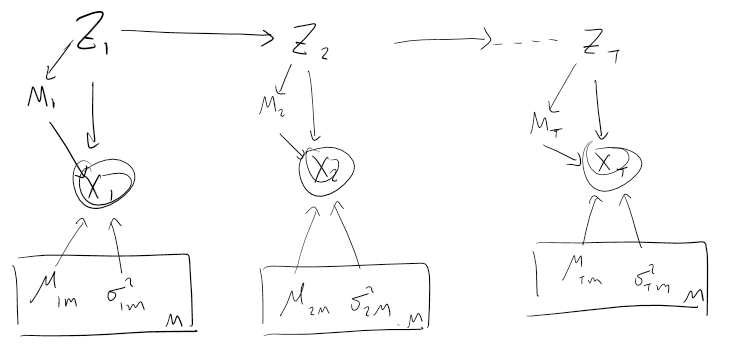
\includegraphics[width=0.7\textwidth]{17.3.png}
  \captionsetup{justification=centering}
  \caption{HMM with Gaussian Mixture per Latent State}
\end{figure*}

\begin{align*}
    p(X_t|Z_t = j, \theta) &= \sum_m w_{jm} \mathcal{N}(X_t|\mu_{jm}, \Sigma_{jm}) \\
    p(X_{1:T}, Z_{1:T}, M_{1:T}) &= p(Z_{1:T}) p(X_{1:T}, M_{1:T}|Z_{1:T}) \\
        &= p(Z_1) \prod_{t=2}^T p(Z_t|Z_{t-1}) \prod_{t=1}^T p(X_t, M_t|Z_t) \\
        &= \prod_{j=1}^K \pi_j^{\mathbb{I}(Z_1=j)}
           \prod_{t=2}^T \prod_{j=1}^K \prod_{k=1}^K A_{jk}^{\mathbb{I}(Z_t=j, Z_{t-1}=k)} 
           \prod_{t=1}^T\prod_{j=1}^K\prod_{m=1}^M p(X_t, M_t|Z_t=j)^{\mathbb{I}(Z_t=j, M_t=m)} \\
    \ell_c(\theta) &= 
       \sum_{j=1}^K N_j^1 \ln \pi_j
       + \sum_{j=1}^K \sum_{k=1}^K N_{jk} \ln A_{jk} 
       + \sum_{j=1}^K\sum_{m=1}^M N_{jm} \ln w_{jm} \\
       & \quad
       + \sum_{i=1}^N \sum_{t=1}^T\sum_{j=1}^K\sum_{m=1}^M \mathbb{I}(Z_{i,t}=j) \mathbb{I}(M_{i,t}=m)
            \ln \mathcal{N}(X_{i,t}|\mu_{jm}, \Sigma_{jm}) \\
    N_j^1 &= \sum_{i=1}^N \mathbb{I}(Z_{i,1}=j) \\
    N_{jk} &= \sum_{i=1}^N \sum_{t=2}^T \mathbb{I}(Z_{i,t}=j, Z_{i,t-1}=k) \\
    N_{jm} &= \sum_{i=1}^N \sum_{t=1}^T \mathbb{I}(Z_{i,t}=j, M_{i,t}=m) \\
\end{align*}

\paragraph{E-step}
Due to the latent variables, we need to use EM or Baum-Welch algorithm. Here we derive the solutions for those determined by $Z$ and $M$ for the E-step. $\gamma$ and $\xi$ are the solutions from the forward-backward algorithm smoothing. And the responsibility $r_{i,t,j,m}$ decompose because it has no time dependency, which results in a usual EM solution conditional on $Z_{i,t}=j$.
\begin{align*}
    Q(\theta, \theta^{t-1}) &= \mathbb{E}[\ell_c(\theta) | X, \theta^{t-1}] \\
        &= \sum_{j=1}^K \mathbb{E}[N_j^1] \ln \pi_j
        + \sum_{j=1}^K \sum_{k=1}^K \mathbb{E}[N_{jk}] \ln A_{jk} 
        + \sum_{j=1}^K\sum_{m=1}^M \mathbb{E}[N_{jm}] \ln w_{jm} \\
        & \quad
        + \sum_{i=1}^N \sum_{t=1}^T\sum_{j=1}^K\sum_{m=1}^M p(Z_{i,t}=j, M_{i,t}=m|X,\theta^{t-1})
            \ln \mathcal{N}(X_{i,t}|\mu_{jm}, \Sigma_{jm}) \\
    \mathbb{E}[N_j^1] &= \sum_{i=1}^N p(Z_{i,1}=j | X_i, \theta^{t-1}) = \sum_{i=1}^N \gamma_{i,1}(j) \\
    \mathbb{E}[N_{jk}] &= \sum_{i=1}^N \sum_{t=2}^{T_i} p(Z_{t-1}=j, Z_t=k|X_i, \theta^{t-1})
        = \sum_{i=1}^N \sum_{t=2}^{T_i} \xi_{i,t}(j, k) \\
    \mathbb{E}[N_{j}] &= \sum_{i=1}^N \sum_{t=1}^{T_i} \sum_{m=1}^M
        p(M_{i,t}=m|Z_{i,t}=j, X_i, \theta^{t-1}) p(Z_{i,t}=j|X_i, \theta^{t-1}) \\
        &= \sum_{i=1}^N \sum_{t=1}^{T_i} \gamma_{i,t}(j) \sum_{m=1}^M r_{i,t,j,m} \\
    \gamma_{i,t}(j) &= p(Z_t=j|X_i, \theta) \\
    \xi_{i,t}(j, k) &= p(Z_{t-1}=j, Z_t=k|X_i, \theta) \\
    r_{i,t,j,m}|Z_{i,t} &=
        \frac{w_{jm} \mathcal{N}(X_{it}|\mu_{jm}, \Sigma_{jm})}
             {\sum_{m'}^M w_{jm'} \mathcal{N}(X_{it}|\mu_{jm'}, \Sigma_{jm'})}
\end{align*}

\paragraph{M-step}
The M-step solutions follow the Baum-Welch results with a sprinkle of GMM results.
\begin{align*}
    \hat{A}_{jk} &= \frac{\mathbb{E}[N_{jk}]}{\sum_{k'} \mathbb{E}[N_{jk'}]} \\
    \hat{\pi}_k &= \frac{\mathbb{E}[N_{k}^1]}{N} \\
    \hat{w}_{jm} &= \frac{\mathbb{E}[N_{jm}]}{\mathbb{E}[N_{j}]} \\
    \hat{\mu}_{jm} &= \frac{\mathbb{E}[\bar{X}_{jm}]}{\mathbb{E}[N_{jm}]} \\
    \mathbb{E}[\bar{X}_{jm}] &=
        \sum_{i=1}^N \sum_{t=1}^{T_i} \gamma_{i,t}(j) \, r_{i,t,j,m} X_{i,t} \\
    \hat{\Sigma}_{jm} &=
        \frac{
            \mathbb{E}[(\bar{XX})^{\intercal}_{jm}]
            - \mathbb{E}[N_{jm}] \hat{\mu}_{jm} \hat{\mu}_{jm}^{\intercal}
        } {\mathbb{E}[N_{jm}]} \\
    \mathbb{E}[(\bar{XX})^{\intercal}_{jm}] &=
        \sum_{i=1}^N \sum_{t=1}^{T_i} \gamma_{i,t}(j) \, r_{i,t,j,m} X_{i,t} X_{i,t}^{\intercal} 
\end{align*}

\newpage
\section{Exercise 17.4}
Here in this question, instead of having $KM$ different Gaussians, we assume that we only have $M$ Gaussians. The latent variable $Z$ only affects the mixture weights $w_jm$.
\begin{figure*}[!h]
  \centering
  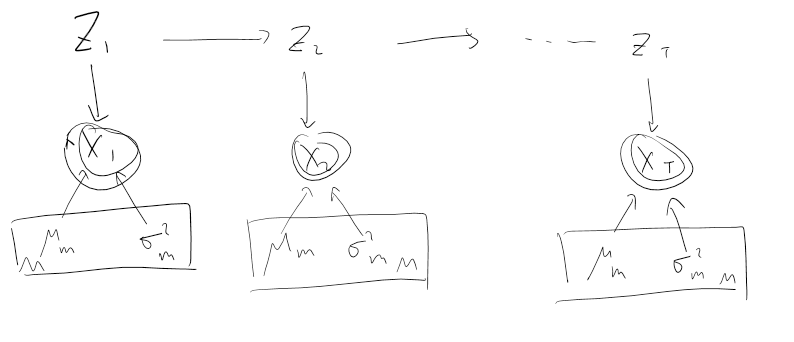
\includegraphics[width=0.7\textwidth]{17.4.png}
  \captionsetup{justification=centering}
  \caption{Semi-Continuous HMM with a Tied Gaussian Mixtures}
\end{figure*}

\paragraph{The E-Step}
Hence, the new observation model and the expected complete data log-likelihood are below, which is very similar to the previous exercise.
\begin{align*}
    p(X_t|Z_t = j, \theta) &= \sum_m w_{jm} \mathcal{N}(X_t|\mu_m, \Sigma_m) \\
    Q(\theta, \theta^{t-1}) &= \mathbb{E}[\ell_c(\theta) | X, \theta^{t-1}] \\
        &= \sum_{j=1}^K \mathbb{E}[N_j^1] \ln \pi_j
        + \sum_{j=1}^K \sum_{k=1}^K \mathbb{E}[N_{jk}] \ln A_{jk} 
        + \sum_{j=1}^K\sum_{m=1}^M \mathbb{E}[N_{jm}] \ln w_{jm} \\
        & \quad
        + \sum_{i=1}^N \sum_{t=1}^T \sum_{j=1}^K p(Z_{i,t}=j|X, \theta^{t-1})
            \sum_{m=1}^M p(M_{i,t}=m|X,\theta^{t-1}) \ln \mathcal{N}(X_{i,t}|\mu_m, \Sigma_m) \\ \\
    \mathbb{E}[N_j^1] &= \sum_{i=1}^N p(Z_{i,1}=j | X_i, \theta^{t-1}) = \sum_{i=1}^N \gamma_{i,1}(j) \\
    \mathbb{E}[N_{jk}] &= \sum_{i=1}^N \sum_{t=2}^{T_i} p(Z_{t-1}=j, Z_t=k|X_i, \theta^{t-1})
        = \sum_{i=1}^N \sum_{t=2}^{T_i} \xi_{i,t}(j, k) \\
    \mathbb{E}[N_{jm}] &= \sum_{i=1}^N \sum_{t=1}^{T_i}
        p(M_{i,t}=m|Z_{i,t}=j, X_i, \theta^{t-1}) p(Z_{i,t}=j|X_i, \theta^{t-1}) \\
        &= \sum_{i=1}^N \sum_{t=1}^{T_i} \gamma_{i,t}(j) r_{i,t,j,m} \\
    \gamma_{i,t}(j) &= p(Z_t=j|X_i, \theta) \\
    \xi_{i,t}(j, k) &= p(Z_{t-1}=j, Z_t=k|X_i, \theta) \\
    r_{i,t,j,m}|Z_{i,t} &=
        \frac{w_{jm} \mathcal{N}(X_{it}|\mu_m, \Sigma_m)}
             {\sum_{m'}^M w_{jm'} \mathcal{N}(X_{it}|\mu_{m'}, \Sigma_{m'})}
\end{align*}

\paragraph{The M-Step} Similarly, the maximization step is also lookalike. Just the new $\mu$ and $\Sigma$ MLE solutions now incorporate all data no matter the latent state were.
\begin{align*}
    \hat{A}_{jk} &= \frac{\mathbb{E}[N_{jk}]}{\sum_{k'} \mathbb{E}[N_{jk'}]} \\
    \hat{\pi}_k &= \frac{\mathbb{E}[N_{k}^1]}{N} \\
    \hat{w}_{jm} &= \frac{\mathbb{E}[N_{jm}]}{\mathbb{E}[N_{j}]} \\
    \hat{\mu}_{m} &= \frac{\mathbb{E}[\bar{X}_{m}]}{\mathbb{E}[N_{m}]} \\
    \mathbb{E}[\bar{X}_{m}] &=
        \sum_{i=1}^N \sum_{t=1}^{T_i} \sum_{j=1}^{K} \gamma_{i, t}(j) r_{i,t,j,m} X_{i,t} \\
    \hat{\Sigma}_{m} &=
        \frac{
            \mathbb{E}[(\bar{XX})^{\intercal}_{m}]
            - \mathbb{E}[N_{m}] \hat{\mu}_{m} \hat{\mu}_{m}^{\intercal}
        } {\mathbb{E}[N_{m}]} \\
    \mathbb{E}[(\bar{XX})^{\intercal}_{m}] &=
        \sum_{i=1}^N \sum_{t=1}^{T_i} \sum_{j=1}^{K} \gamma_{i,t}(j) \, r_{i,t,j,m} X_{i,t} X_{i,t}^{\intercal} 
\end{align*}

\section{AQ 1}
Given the transition matrix $A$ with 5 states $\{A, B, C, D, E\}$, it has the following properties.
\paragraph{Communicating class}
\begin{enumerate}
  \item $c_1 = \{A, E\}$
  \item $c_2 = \{B, D\}$
  \item $c_3 = \{C\}$
\end{enumerate}

\paragraph{Recurrent & Transient}
\begin{enumerate}
  \item Recurrent: $\{A, E, C\}$
  \item Transient: $\{B, D\}$
\end{enumerate}

\paragraph{Stationary Distribution}
\begin{bmatrix}
    \frac{1}{2} & 0 & 0 & 0 & \frac{1}{2} \\
    \frac{1}{4} & 0 & \frac{1}{2} & 0 & \frac{1}{4} \\
    0 & 0 & 1 & 0 & 0 \\
    \frac{1}{4} & 0 & \frac{1}{2} & 0 & \frac{1}{4} \\
    \frac{1}{2} & 0 & 0 & 0 & \frac{1}{2} \\
\end{bmatrix}

\section{AQ 2}
Under a time-invariant homogeneous Markov Chain, the transition matrix $A$ is time-invariant. Therefore, we have the Chapman-Kolmogorov property.
\begin{align*}
    A_{ij}(n) &= p(X_{t+n}=j|X_{t}=i) \\
    A(m+n) &= A(m) A(n) \\
    A(n) &= A A(n-1) = A A A(n-2) = \dots = A^n
\end{align*}

Hence, if we have a $X_0, X_1, X_2, \dots$ Markov Chain with a transition matrix $P$ and a initial state $\pi_o$. Then a new chain $Y_t = X_{kt}$ that every step moves $k$ steps equivalently in X has a transition matrix $P^k$
\begin{align*}
    X_{kt-k+1} &= X_{kt-k} P \\
    X_{kt-k+2} &= X_{kt-k} P^2 \\
    & \dots \\
    X_{kt} &= X_{kt-k} P^k \\
    Y_t &= X_{kt-k} P^k \\
    Y_t &= \pi_o P^{kt} \\
\end{align*}

\section{AQ 3}
We can just brutal force it by constructing the transition matrix $A$ with 6 finite states because we have $3!$ possible ordering given 3 books. The probability of choosing each book $i \in \{1, 2, 3\}$ is given by $a_i > 0$.
\begin{align*}
    \begin{bmatrix}
        a_1 & 0 & a_2 & 0 & a_3 & 0 \\
        0 & a_1 & a_2 & 0 & a_3 & 0 \\
        a_1 & 0 & a_2 & 0 & 0 & a_3 \\
        a_1 & 0 & 0 & a_2 & 0 & a_3 \\
        0 & a_1 & 0 & a_2 & a_3 & 0 \\
        0 & a_1 & 0 & a_2 & 0 & a_3 \\
    \end{bmatrix}
\end{align*}
The chain is finite and is certainly irreducible and aperiodic. Aperiodicity can be proven easily based on that each state has a self loop, the diagonals; hence, $gcd\{t:A_{ii}(t) > 0\} = 1$. And we can certainly see the chain is strongly connected because the $P_{ij}(t) > 0, \, \forall i, j \in K, \, t > 0$.

\end{document}